%%%%%%%%%%%%%%%%%%%%%%%%%%%%%%%%%%%%%%%%%%%%%%%%%%%%%%%%%%%%%%%%%%%%%%%%%%%%%%%

\chapter{Einleitung}
Dieser Praxisbericht thematisiert das Messen von Schiffsemissionen durch den Emissionsmesser MARSIC300, der SICK AG. Dabei wird der technische Rahmen um die Entstehung und Filterung von Schiffsemissionen erläutert woraufhin beschrieben wird weshalb, die Messung von Schiffsemissionen zwingend erforderlich ist im Hinblick auf regulatorische und rechtliche Aspekte. Auch soll ein genauerer Einblick in die Funktionsweise des MARSIC300 gegeben werden, so wie auch die Kozeptionierung von Anwendungsmöglichkeiten im Bezug auf Servicedienstleistungen durch die Analyse von gesammelter Big Data, mit der Hilfe von marinetraffic.com. Die Ergebnisse werden darauf hin evaluiert und ein Ausblick zur zukünftigen Weiterentwicklung wird gegeben. Diese Praxisarbeit dient unter anderem zur theoretischen Vorbereitung auf die Bachelorarbeit. 
%%%%%%%%%%%%%%%%%%%%%%%%%%%%%%%%%%%%%%%%%%%%%%%%%%%%%%%%%%%%%%%%%%%%%%%%%%%%%%%

\section{Projektumfeld}

%%%%%%%%%%%%%%%%%%%%%%%%%%%%%%%%%%%%%%%%%%%%%%%%%%%%%%%%%%%%%%%%%%%%%%%%%%%%%%%

\subsection{Firma}
Das Unternehmen Sick AG wurde 1946 von Erwin Sick gegründet und zählt mit einer Vielzahl von Sensorlösungen vor allem in der Fabrik-, Logistik- und Prozessautomation zum Markt- und Technologieführer für Sensorintelligenz. Die Sick AG ist global in über 80 Ländern mit 50 Tochtergesellschaften vertreten und beschäftigt weltweit über 10.000 Mitarbeiter. Dabei wächst das Unternehmen stetig und erwirtschaftete beispielweise im Geschäftsjahr 2019 einen Umsatz von rund 1,8 Mrd. Euro\cite{SICK.2021a}.
\begin{figure}[H]
\centering
\fbox{\includegraphics[height=0.15\textheight]{Bilder/SickFirmenGebäude}}
\caption{\label{fig-firmenHQ}Der Firmen Sitz der Sick AG in Waldkirch}
\end{figure}
%%%%%%%%%%%%%%%%%%%%%%%%%%%%%%%%%%%%%%%%%%%%%%%%%%%%%%%%%%%%%%%%%%%%%%%%%%%%%%%
\subsection{Abteilung}
Das Global Industrie Center Process Automation unterteilt sich in 5 Untersegmente mit den Schwerpunkten Basic Materials, Infrastructure, Oil and Gas, International Tender Management und Area sales support. Die teilweise wiederum Unterteilt werden können. 
\begin{figure}[H]
\centering
\fbox{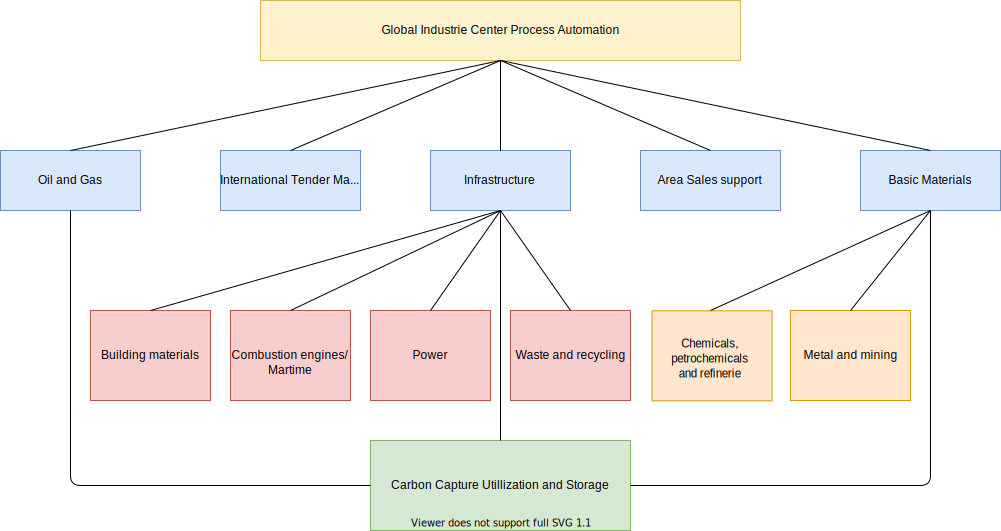
\includegraphics[height=0.4\textheight]{Bilder/Organigramm_GICPA}}
\caption{\label{fig-firmenOG}Das Organigramm der GICPA}
\end{figure}
Das Projekt findet dabei in der Abteilung mit dem Schwerpunkt Comubustion enginnes/Maritime unter der Leitung von Hinrich Brumm statt. Primäre Aufgabe der Gruppe ist es effiziente Lösungen für Industrien mit dem Schwerpunkt auf Verbrennung Prozessen zu finden. Beispiele wäre dabei eben die Verbrennung von Diesel. 
%%%%%%%%%%%%%%%%%%%%%%%%%%%%%%%%%%%%%%%%%%%%%%%%%%%%%%%%%%%%%%%%%%%%%%%%%%%%%%%

\section{Motivation}

%%%%%%%%%%%%%%%%%%%%%%%%%%%%%%%%%%%%%%%%%%%%%%%%%%%%%%%%%%%%%%%%%%%%%%%%%%%%%%%

